\subsubsection{Data Model}
When planning the implementation of the server we decided to use a MSSQL database to store our data. Then we spent hours considering different scenarios and arranging the entities into the following data model.
\begin{figure}[H]
  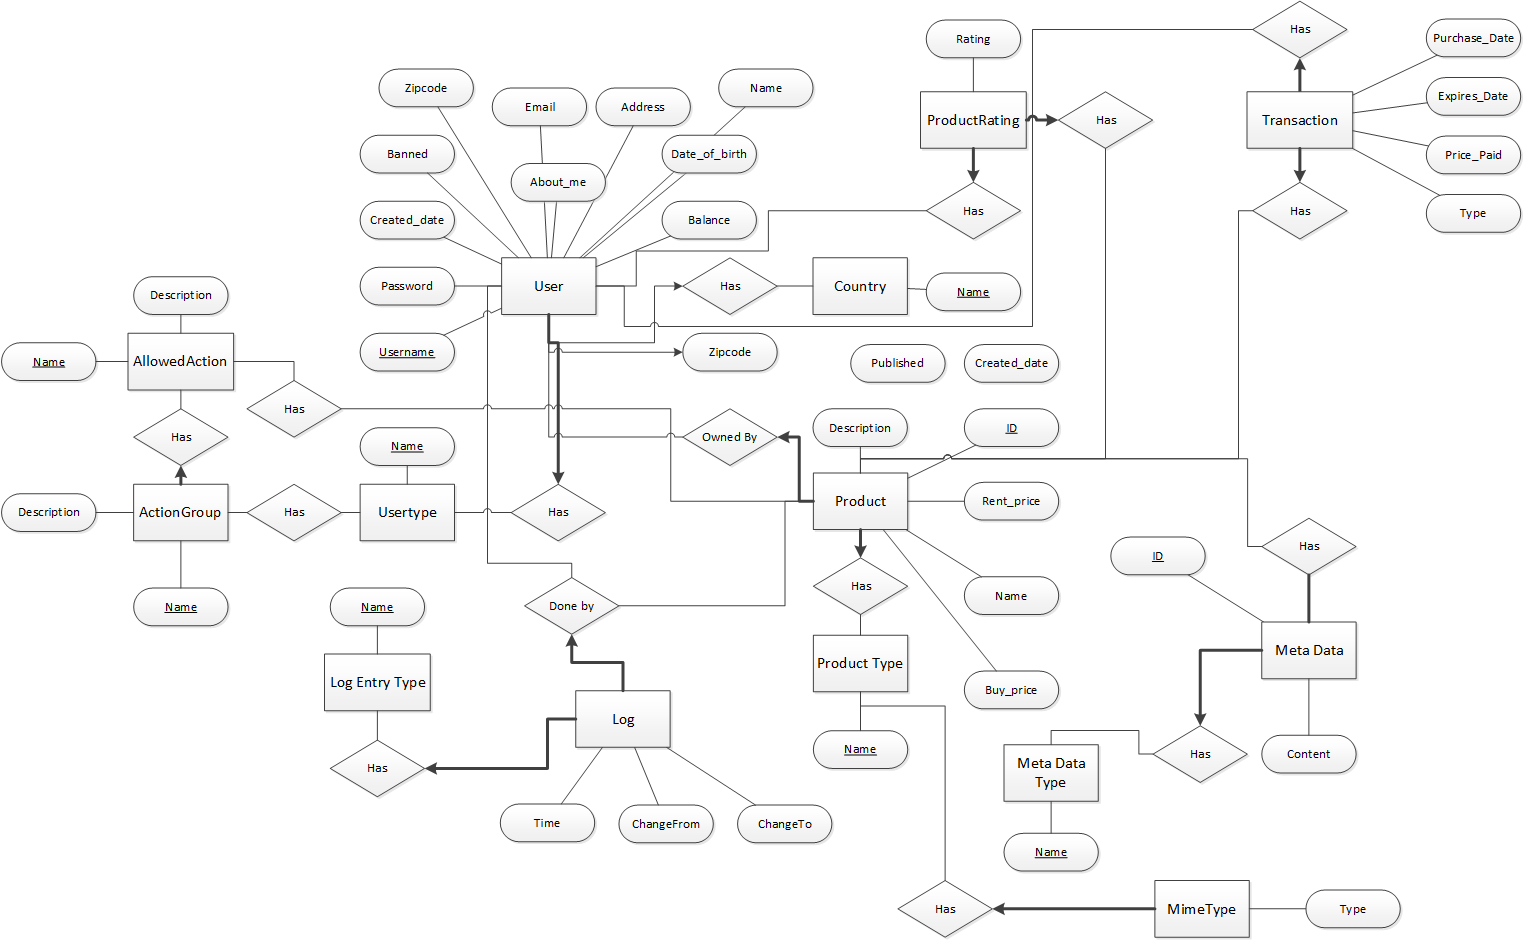
\includegraphics[width=\textwidth]{illustrations/Datamodel.png}
  \caption{Our data model as used by the database}
  \label{fig:datamodel}
\end{figure}
We will now explain the different entities and their purpose in our system.

\begin{description}
\item[User] \hfill \\
Our first and possibly most important entity is the User entity. It contains information regarding each user of our system. Each user also has an optional \todo{optional country sounds weird}{Morten} country, referenced through the Country entity explained later.

Furthermore, the User entity has a relation to the Usertype entity. Having Usertype as a separate entity as opposed to simply an attribute makes it possible for us to create relations to the type and not each individual user. For instance we have a relation between Usertype and ActionGroup, explained later.

\item[Country] \hfill \\
Each user can have a country defined. The reason we modeled this as a separate entity is so that the user can select their country from a list of available ones.

\item[Usertype] \hfill \\
The user type defines which type the user is. The possible values in our program is:
\begin{itemize}
	\item Customer
	\item Content Provider
	\item Admin
\end{itemize}

Each user type has zero-to-many action groups. The function of that entity is explained later.

\item[ActionGroup] \hfill \\
An action group is a way to gather permissions in a group. This way we avoid having to give a lot of permissions to each user type. Our initial idea was to create action groups having names like `View general data', `Create and edit products' and `Administer products'. This would make it easy to create a new user type like `Content moderator' and assign groups of permissions at a time.

Our implementation was not like this though. We ended up making this entity completely useless as we created the exact same action groups as we had user types.

\item[AllowedAction] \hfill \\
Our AllowedAction entity is our way of defining permissions in the system. Whenever you need to check whether or not a user has permission to do something in our system you check the allowed action name (an example could be BAN\_UNBAN\_ANY).

The allowed action is referenced by both the ActionGroup entity and the Product entity. This is because we have chosen to model whether or not products should be buyable or rentable in our permissions system. Products can therefore have BUYABLE and RENTABLE allowed actions.

\item[Product] \hfill \\ 
Product is our main entity for storing information about a product such as a movie, an ebook, etc. It has some base information about a product. It also has a product type. This is through the ProductType entity as described later.

There are three other entities which refer to Products, all described later:
\begin{itemize}
	\item MetaData
	\item ProductRating
	\item Transaction
\end{itemize}

\item[ProductType] \hfill \\
Each product has a product type. The product type is used to semantically separate the different types of products. Furthermore, it references another entity called MimeType.

\item[MimeType] \hfill \\
MimeType is used to limit which files can be uploaded for a specific product type. When creating a product you choose which type it is of. As it makes no sense to upload a PDF-file for a product of type `movie' we chose to limit this using the information stored here.

\item[MetaData] \hfill \\
A product can have zero-to-many meta data attached. This can be used to describe things that are specific to the particular product, like pages for an ebooks or duration for a movie. Each meta data has a reference to the MetaDataType entity.

\item[MetaDataType] \hfill \\
The MetaDataType entity is used to control meta data. If users were to enter meta data, we would like to limit which types they are able to enter, to avoid things like `length', `Length', `LENgTh' and `Lengt' which are basically the same thing. It would also make search more versatile, as you, in theory, could search for movies with a length of more than 1 hour.

\item[ProductRating] \hfill \\
This is used to store ratings that users have given products. Each user can only have one rating on each product. If a users tries to vote more than once, their vote should be updated.

We have defined ratings to be from -5 to 5. This means that users can be positive or negative towards a product.

\item[Transaction] \hfill \\
Our Transaction entity represents a finished customer purchase. It records the information needed by our system for a purchase. If it is a rent the expire date is also stored here.

\item[Log] \hfill \\
While we planned our entire data model we wanted to make everything loggable. It is important to be able to monitor the system and the activity herein, especially for legal reasons. Furthermore, our implementation would make it possible to revert things to previous states.

Each entry has a type, which is defined in the LogEntryType entity.

\item[LogEntryType] \hfill \\
This entity was planned to make searching through log entries easier. If we wanted to know how many people have logged in this year we could just take the log entries of type `login' and count them.
\end{description}